\documentclass{report}
\usepackage[spanish]{babel}



\usepackage[spanish]{babel}
\usepackage[utf8x]{inputenc}
\usepackage{amsmath}
\usepackage{graphicx}
\usepackage[colorinlistoftodos]{todonotes}
\usepackage{enumitem}
\usepackage{listings}
\usepackage{verbatim}
\usepackage{eurosym}
\usepackage[export]{adjustbox}
\usepackage{amssymb}
\usepackage{bussproofs}
\usepackage{amsmath}
\usepackage{tikz}
\usepackage{xcolor}
\usepackage{listings}
\usepackage{titletoc}
\usepackage{hyperref}

\hypersetup{
  colorlinks=true,
  linkcolor=black,
  urlcolor=blue,
  citecolor=black
}

\newcommand{\coverPage}[6]{%
%----------------------------------------------------------------------------------------
%	COVER START
%----------------------------------------------------------------------------------------
\begin{titlepage}

    \newcommand{\HRule}{\rule{\linewidth}{0.5mm}}
    \newcommand{\department}{#1}
    \newcommand{\course}{#2}
    \newcommand{\titleValue}{#3}
    \newcommand{\subtitleValue}{#4}
    \newcommand{\authorName}{#5}

    \center

    %----------------------------------------------------------------------------------------
    %	HEADER
    %----------------------------------------------------------------------------------------
    
\includegraphics{images/logo_usa.png}
    \vspace{0.5cm}
    \textsc{\Large \department}\\[0.5cm]
    \textsc{\Large \course}\\[0.5cm]
    \vfill

    %----------------------------------------------------------------------------------------
    %	TITLE
    %----------------------------------------------------------------------------------------

    \HRule\\
    \Huge
    \textbf{\titleValue}\\[0.5cm]
    \Large
    \textbf{\subtitleValue}\\
    \HRule\\[0.5cm]

    %----------------------------------------------------------------------------------------
    %	AUTHOR AND DATE
    %----------------------------------------------------------------------------------------

    \vfill
    \Large
    \textit{\authorName}\\
    {\large \today}\\[2cm]

\end{titlepage}
%----------------------------------------------------------------------------------------
%	COVER END
%----------------------------------------------------------------------------------------
}

\begin{document}
    \coverPage{ Matemáticas }{ Cálculo Diferencial }{ Tarea 3 }{  }{ Alexander Mendoza \\ Dylan Cifuentes }{\today}

    \pagebreak
    \subsection*{Tarea 3}
    \begin{enumerate}
        \item Demuestre la fórmula de Cauchy: Sean $f$ y $g$ dos funciones continuas en un intervalo cerrado $\left[a,b\right]$ y derivables en $\left(a, b\right)$. Entonces para un cierto $c \in \left(a, b\right)$, tenemos

        $$f'(c)\left[g(b)-g(a)\right] = g'(c)\left[f(b)-f(a)\right]$$

        \textit{\textbf{Demostración}}. Sea \(h(x) = f(x)[g(b) - g(a)] - g(x)[f(b) - f(a)]\). Observamos que \(h\) es continua en \([a, b]\), diferenciable en \((a, b)\), y que
        \begin{align*}
            h(a) &= f(a)[g(b) - g(a)] - g(a)[f(b) - f(a)] \\
            &= [f(a)g(b) - f(a)g(a)] - [g(a)f(b) - g(a)f(a)] \\
            &= [f(a)g(b) - g(a)f(a)] - [g(a)f(b) - g(a)f(a)] \\
            &= f(a)g(b) - g(a)f(b)
        \end{align*}

        Además tenemos que la derivada de $h(x)$ es la siguiente

        \[ h'(x) = f'(x)[g(b) - g(a)] - g'(x)[f(b) - f(a)] \]

        Luego, por el Teorema de Rolle, existe \(c\) en \((a, b)\) tal que \(h'(c) = 0\). Al tomar \(h'(c) = 0\), tenemos lo siguiente

        \[ 0 = f'(c)[g(b) - g(a)] - g'(c)[f(b) - f(a)] \]

        De esta manera tenemos que
        \begin{align*}
            f'(c)[g(b) - g(a)] = g'(c)[f(b) - f(a)]
        \end{align*}

        \item Probar que $x^2=x\sin(x)+\cos(x)$ se verifica exactamente para dos valores de $x$.\\
        \textit{\textbf{Demostración}}. Reescribiremos la ecuación como $f(x)=x^2-x\sin(x)-\cos(x)=0$, luego hallemos sus puntos críticos, entonces:\\
        $f'(x)=x^2-x\sin(x)-\cos(x)= 2x-\sin(x)-x\cos(x)+\sin(x)=2x-x\cos(x)=x(2-\cos(x))$.\\
        Notemos que $(2-\cos(x))$ nunca se hace $0$, luego si $x=0$, este es su único punto crítico.
        Además, si $x<0$, entonces $f'(x)<0$, por tanto $f$ decrece. Si $x>0$, entonces $f'(x)>0$, por tanto $f$ crece. Por tanto, $x=0$ es un mínimo relativo.
        Por último, veamos que $f(x)=f(-x)$, es decir, $f$ es par.\\
        Demostración: Probemos que no existen puntos $x_1,x_2,...,x_i$ positivos tales que $f(x_i)=0$ para todo $i\geq 2$, además supongamos que $x_i< x_{i+1}$.
        Por el teorema de valor medio, existe un $\beta_i \in (x_i,x_{i+1})$ tal que $f(\beta_i)=0$ con $i\geq2$, luego existe más de un punto crítico, lo que contradice nuestra hipótesis inicial de que $x=0$ es el único punto crítico.\\
        Luego, o existe un $\alpha\in \mathbb{R}$ tal que  $\alpha>0$ y $f(\alpha)=0$, o no existe ese $\alpha$.\\
        Para probar su existencia, tomemos $x=0$ y $x= \pi$, si reemplazamos en $f$, tenemos que:\\
        $f(0)=-1$ y $f(\pi)=\pi^2+1$.\\
        Puesto que $f$ es creciente y continua con $x>0$, entonces existe algún $\alpha \in (0,\pi)$ que cumple que $f(\alpha)=0$. Como sabemos que $f$ es par, entonces también se debe cumplir para $-\alpha$, por tanto, hemos hallado nuestros dos valores.

        \item Dibuje la gráfica de $f(x)= \dfrac{x^2(x+1)^3}{(x-2)^2(x-4)^4}$\\
        \begin{itemize}
            \item Dom: $(\infty, 2) \cup (2,4) \cup (4, \infty)$
            \item Asíntota vertical: $x=2, x=4$
            \item Asíntota horizontal: $x=0$
            \item $f'(x)=  -\dfrac{x (x+1)^2 (x^3 + 18x^2 - 44x - 16)}{(x-2)^3 (x-4)^5)}$
            \item  $f'(x)=0$ si $x=-20.14476, x=-1, x=-0.321983, x=0,x= 2.46675 $\\
            \item $f'(x)$ no existe si $x=2, x=4$
            $(-\infty, -20.14476)$ decreciente\\
            $(-20.14476, -1)$ Crece,
            $(-1,-0.321983)$ Crece,
            $(-0.321983, 0)$ Decrece,
            $(0,2)$ Crece,
            $(2,2.46675)$ Crece,
            $(2,4)$ Decrece.
            \item $f''(x)=\dfrac{2 (x^7 + 37 x^6 + 42 x^5 - 622 x^4 + 56 x^3 + 1356 x^2 + 736 x + 64)}{(x-2)^4 (x-4)^6)}$
            Puntos de inflexión:
            \\$f''(x)=0$ si $x=-35.3113,x=-4.97777, x=-1, x=-0.542718, x=-0.108386$\\
            $(-\infty, -35.3113)$ Concava $,
            (-35.3113,4.97777)$ Convexa $,
            (-4.97777,-1)$ Concava $,\\
            (-1, -0.542718)$ Convexa$,
            (-0.542718,-0.108386 )$ Concava $,
            (-0.108386, \infty)$ Convexa.
            \item Cortes con eje x; $(-1,0), (0,0) $
            \item Corte con eje y; $(0,0)$
            \item $\lim_{x->2^+} \frac{x^2 (x + 1)^3)}{(x - 2)^2 (x - 4)^4} = \infty$, $\lim_{x->2^-} \frac{x^2 (x + 1)^3)}{(x - 2)^2 (x - 4)^4} = \infty$
            \item $\lim_{x->4^+} \frac{x^2 (x + 1)^3)}{(x - 2)^2 (x - 4)^4} = \infty$, $\lim_{x->4^-} \frac{x^2 (x + 1)^3)}{(x - 2)^2 (x - 4)^4} = \infty$
            \item $\lim_{x->\infty} \frac{x^2 (x + 1)^3)}{(x - 2)^2 (x - 4)^4} = 0$, $\lim_{x->-\infty} \frac{x^2 (x + 1)^3)}{(x - 2)^2 (x - 4)^4} = 0$
    
    Este es el codigo por si te queda más facil pasarlo

            Con esto tenemos la siguiente grafica

            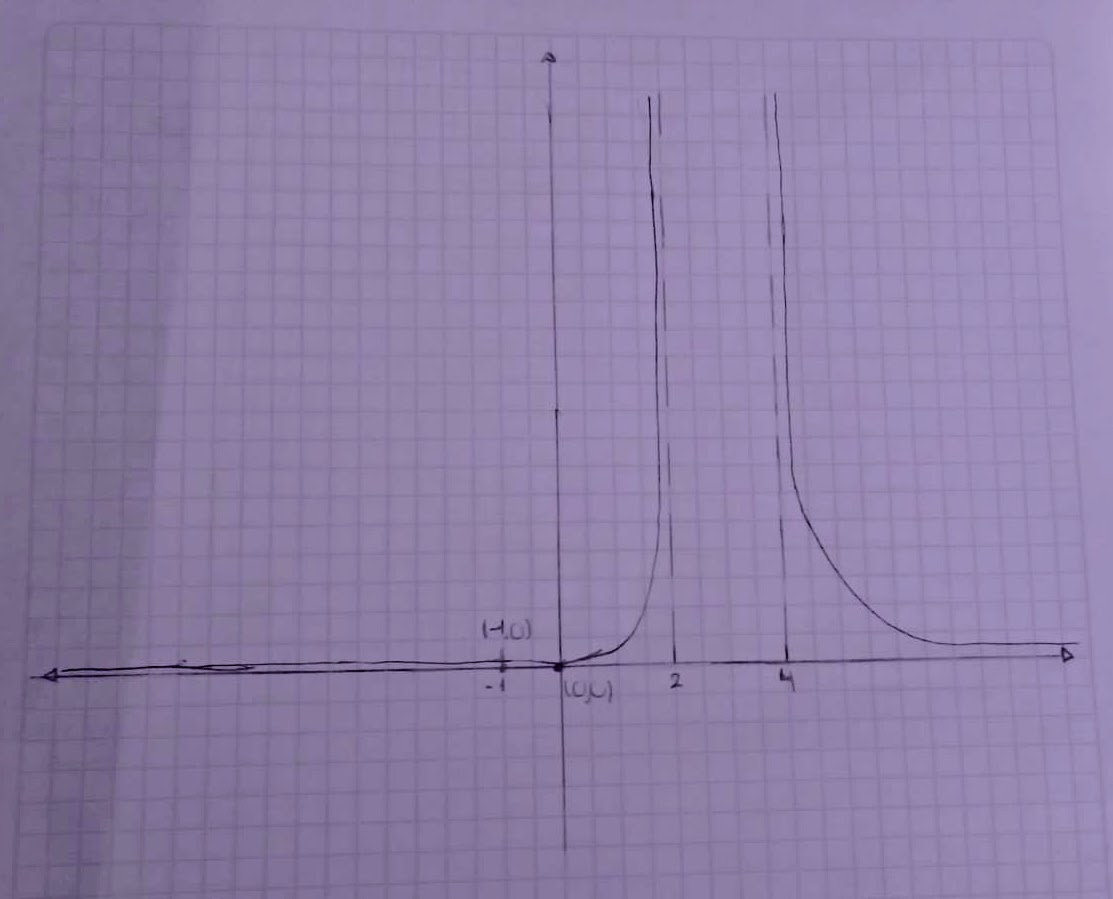
\includegraphics[width=1\textwidth]{images/grafica.jpeg}
        \end{itemize}

        \item Demuestre que si $f$ es continua y uno a uno en un intervalo, entonces $f^{-1}$ es también continua.

        \textit{\textbf{Teorema 1}}. Si $f$ es continua e inyectiva sobre un intervalo, entonces $f$ o crece o decrece dentro de ese intervalo.

        \textit{\textbf{Demostración}}. Por el Teorema 1, sabemos que $f$ crece o decrece sobre el intervalo. Supongamos que $f$ es creciente. Sea $b = f(a)$ para algún $a$ en el dominio de $f^{-1}$. Para cualquier $\epsilon > 0$, buscamos $\delta > 0$ tal que si $f(a) - \delta < x < f(a) + \delta$, entonces $a - \epsilon < f^{-1}(x) < a + \epsilon$.

        Elegimos $\delta$ de modo que $\delta = \min\{f(a + \epsilon) - f(a), f(a) - f(a - \epsilon)\}$. Esto asegura que $f(a - \epsilon) \leq f(a) - \delta$ y $f(a) + \delta \leq f(a + \epsilon)$.

        Si $f(a) - \delta < x < f(a) + \delta$, entonces $f(a - \epsilon) < x < f(a + \epsilon)$. Dado que $f$ es creciente, se sigue que $f^{-1}(f(a - \epsilon)) < f^{-1}(x) < f^{-1}(f(a + \epsilon))$, esto es, $a - \epsilon < f^{-1}(x) < a + \epsilon$. Para el caso en el que $f$ es decreciente se puede verificar de la misma forma usando $-f$.

        Por lo tanto, $\lim_{x \to b} f^{-1}(x) = f^{-1}(b)$.

        \item Encuentre la derivada de:

        \begin{enumerate}[label=\alph*)]
            \item $f(x) = \sin(\sin(x))$
            \begin{align*}
                f'(x) &= \frac{d}{dx}[\sin(\sin(x))] \\
                &= \cos(sin(x))\frac{d}{dx}(\sin(x)) \\
                &= \cos(\sin(x)cos(x))
                \end{align*}

            \item $y = \dfrac{1}{(1 + \tan(x))^2}$
            \begin{align*}
                y' &= \frac{1}{(1 + \tan(x))^2} \\
                &= (1 + \tan(x)^{-2}) \\
                &= -\frac{2}{(1 + \tan(x))^3} \frac{d}{dx}(1\tan(x)) \\
                &= -\frac{2}{(1 + \tan(x))^3} \sec^2(x) \\
                &= -\frac{2\sec^2(x)}{(1 + \tan(x))^3}
            \end{align*}

            \item $y = \arctan(x^2 + 1)$
            \begin{align*}
                y' &= \arctan(x^2 + 1) \\
                &= \frac{1}{(x^2 + 1)^2 + 1} \frac{d}{dx}(x^2 + 1) \\
                &= \frac{1}{(x^2 + 1)^2 + 1} \cdot 2x \\
                &= \frac{2x}{x^4 + 2x^2 + 2}
            \end{align*}
            \item $(\cos(x))^x$
            \begin{align*}
                \frac{d}{dx}((\cos(x))^x) &= e^{x\ln(\cos(x))} \frac{d}{dx}(x\ln(\cos(x))) \\
                &= e^{x\ln(\cos(x))}(\ln(\cos(x)) - x\tan(x)) \\
                &= \cos^x(x)(\ln(\cos(x)) - x\tan(x))
            \end{align*}
        \end{enumerate}

        \item Una función $f$ se define como

        $$
            f(x) = \begin{cases}
                x^2 & x\leq c\\
                ax + b & x > c
            \end{cases}
        $$

        Encuentre $a$ y $b$ de manera que $f'(c)$ exista.

        \textit{\textbf{Teorema 2}}. Si $f$ es diferenciable en $a$, entonces $f$ no es continua en $a$.

        \textit{\textbf{Demostración}}. Sabemos que para que una función sea diferenciable, esta debe ser continua (esto se verifica con el contra-recíproco del Teorema 2). Para que $f$ sea continua se debe cumplir lo siguiente

        \begin{align*}
            \lim_{x\to c^-}f(x) &= \lim_{x\to c^+}f(x) \\
        \end{align*}

        Con esto, tenemos que

        \begin{align*}
            \lim_{x\to c^-}x^2 &= \lim_{x\to c^+}ax+b \\
        \end{align*}

        Esto ya que si $x \to c^-$, entonces $x < c$ y si $x \to c^+$, entonces $x > c$. Así se comprueba lo siguiente

        \begin{align*}
            \lim_{x\to c^-}x^2 &= \lim_{x\to c^+}ax+b \\
            c^2 &= ac+b && \text{Por continuidad de funciones.}\\
            b &= c^2 - ac
        \end{align*}

        Comprobemos ahora el valor de $a$ para que $f'(c)$ exista. Para esto debemos verificar que la derivada por izquierda y por derecha de $c$ existan y sean iguales.

        \begin{align*}
            \lim_{h \to 0^-} \dfrac{f(c+h)-f(c)}{h} &= \lim_{h \to 0^+} \dfrac{f(c+h)-f(c)}{h} \\
            \lim_{h \to 0^-} \dfrac{[a(c+h)+b]-c^2}{h} &= \lim_{h \to 0^+} \dfrac{(c+h)^2-c^2}{h} \\
            \lim_{h \to 0^-} \dfrac{[a(c+h)+(c^2-ac)]-c^2}{h} &= \lim_{h \to 0^+} \dfrac{[(c+h)+c][(c+h)-c]}{h}\\
            \lim_{h \to 0^-} \dfrac{ac+ah+c^2-ac-c^2}{h} &= \lim_{h \to 0^+} \dfrac{h(2c+h)}{h}\\
            \lim_{h \to 0^-} \dfrac{ah}{h} &= \lim_{h \to 0^+} \dfrac{h(2c+h)}{h}\\
            a &= 2c
        \end{align*}

        Reemplazando en $b$, tenemos que $b = -c^2$.
    \end{enumerate}
\end{document}
